\chapter{Grundlagen zu auftragsbezogenen Instandhaltungsprozessen}
\markboth{2 Grundlegende Begriffe}{}
\setcounter{footnote}{4}  %um durchgehende Fußnotennummerierung zu haben, hier die Anzahl der bisherigen Fußnoten eintragen

\section{Einordnung in die Produktionswirtschaft}

Bei Instandhaltungsprozessen (engl. maintenance-repair-and-overhaul (MRO)) handelt es sich um einen nachgelagerten Prozess im gesamten Wertschöpfungsprozess der Produktionswirtschaft.\footnote{Vgl. \cite{???}, S. ???.}

Bei dem Begriff der Produktionswirtschaft handelt sich um ein Teilgebiet der Betriebswirtschaftslehre.\footnote{Neben der Teilgebiete Finanzwirtschaft, Marketing, Unternehmensführung, Unternehmensrechnung etc., vgl. dazu \cite{Dyckhoff2010}, S. 3.} In der Produktionswirtschaft wird der Fokus auf die Produktion von Leistung gelegt. Bei diesem ökonomischen Konzept wird die Transformation von materiellen und nichtmateriellen Inputgütern (Produktionsfaktoren) hin zu gewünschten Outputgütern (Leistung des Unternehmens) betrachtet. Bei den im Laufe der Zeit erweiterten betriebswirtschaftlichen Produktionsfaktoren nach \cite[][S. 71]{Gutenberg:1959aa} handelt es sich um   die Elementarfaktoren Werkstoffe, Betriebsstoffe, Betriebsmittel und objektezogene humane Arbeitsleistung sowie um die dispositiven Faktoren Betriebsführung, Organisation und Planung.\footnote{Vgl. \cite{Mitter:1994aa}, S. 27.} Bei Outputgütern handelt es sich um Produkte in Form von Sach- oder Dienstleistungen die dem Markt und somit der potentiellen Nachfrage der Marktteilnehmer zur Verfügung gestellt werden.\footnote{Vgl. \cite{Schmidt:2012aa}, S. 1.} Die Transformation erfolgt durch bestimmte von Menschen veranlasste unternehmerischen Verfahrensweisen.\footnote{Vgl. \cite{tempelmeier1994produktion}, S. 6, echt?????} Beispielsweise kann hier die industrielle Fertigung von Verbrauchs- oder Gebrauchsgütern genannt werden.

%Produktionssysteme?

Bei der Transformation der Inputgüter erfolgt eine qualitative, quantitative, räumliche oder zeitlichen Veränderung der Objekte.\footnote{Vgl. \cite{Dyckhoff2010}, S. 3.} Durch diese Veränderung kann seitens des Unternehmens eine Leistung auf dem Markt angeboten werden. Damit diese Leistung den Absatz bei potentiellen Konsumenten findet, muss die Leistung durch die Transformation eine Wertschöpfung erhalten. Der konzeptionelle Rahmen dieses Gedankens bildet die Wertschöpfungslehre (engl. suppy chain management (SCM)).\footnote{Vgl. \cite{???}, S. ??.} Danach sollte das Ziel eines jeden Unternehmens das Betreiben von Wertschöpfung sein.\footnote{Vgl. \cite{???}, S. ??.} In der klassischen Auffassung der Wertschöpfungslehre durchläuft die Leistungserstellung alle (Teil-)Systeme des Unternehmens.\footnote{???} Abbildung \ref{Prozess} zeigt in Teil a. eine mögliche Abfolge der Systeme eines Unternehmens. Eine klassische Abfolge zur Leistungserstellung bzw. der Transformation von Inputgütern hin zu Outputgütern ist die Abfolge der Systeme Forschung/Entwicklung, Beschaffung, Produktion, Distribution sowie Verkauf. Damit ist die um die Wertschöpfung erhöhte Leistung auf dem Markt angekommen und das Unternehmen erzielt damit i. d. R. einen Ertrag (Revenue).

Sofern das Unternehmen eine \textbf{Instandhaltung} ihrer Leistungen anbieten kann, wird die Abfolge des Wertschöpfungsprozesses um dieses Unternehmenssystem erweitert. Für den gewerblichen Verkauf von Gütern an Privatkunden können gesetzliche Regelungen bestehen, womit ein Unternehmen gezwungen ist das Unternehmenssystem der Instandhaltung in den Wertschöpfungsprozess aufzunehmen.\footnote{Vgl. die Richtlinie 1999/44/EG des Europäischen Parlaments und des Rates vom 25. Mai 1999 zu bestimmten Aspekten des Verbrauchsgüterkaufs und der Garantien für Verbrauchsgüter.}

Nach der DIN 310511 wird Instandhaltung insofern ausgeführt, wenn die Funktionsfähigkeit der Leistung eines Unternehmens sichergestellt werden muss, damit der ursprüngliche Wert erhalten bleibt.\footnote{Vgl. \cite{Strunz:2012aa}, S. 1.} 

Definitionen gemäß DIN 31051:
\begin{itemize}
\item Instandhaltung ist die Kombination aller technischen und administrativen Maßnahmen des Managements während des Lebenszyklus einer Betrachtungseinheit zur Erhaltung des funktionsfähigen Zustandes oder der Rückführung in diesen, so dass sie die geforderte Funktion erfüllen kann.
\item Als Betrachtungseinheit (BE) wird jedes Bauelement, Gerät, Teilsystem, jede Funktionseinheit, jedes Betriebsmittel oder System, das für sich allein betrachtet werden kann, definiert.
\end{itemize}

\begin{figure}[h!]
  \begin{center}
    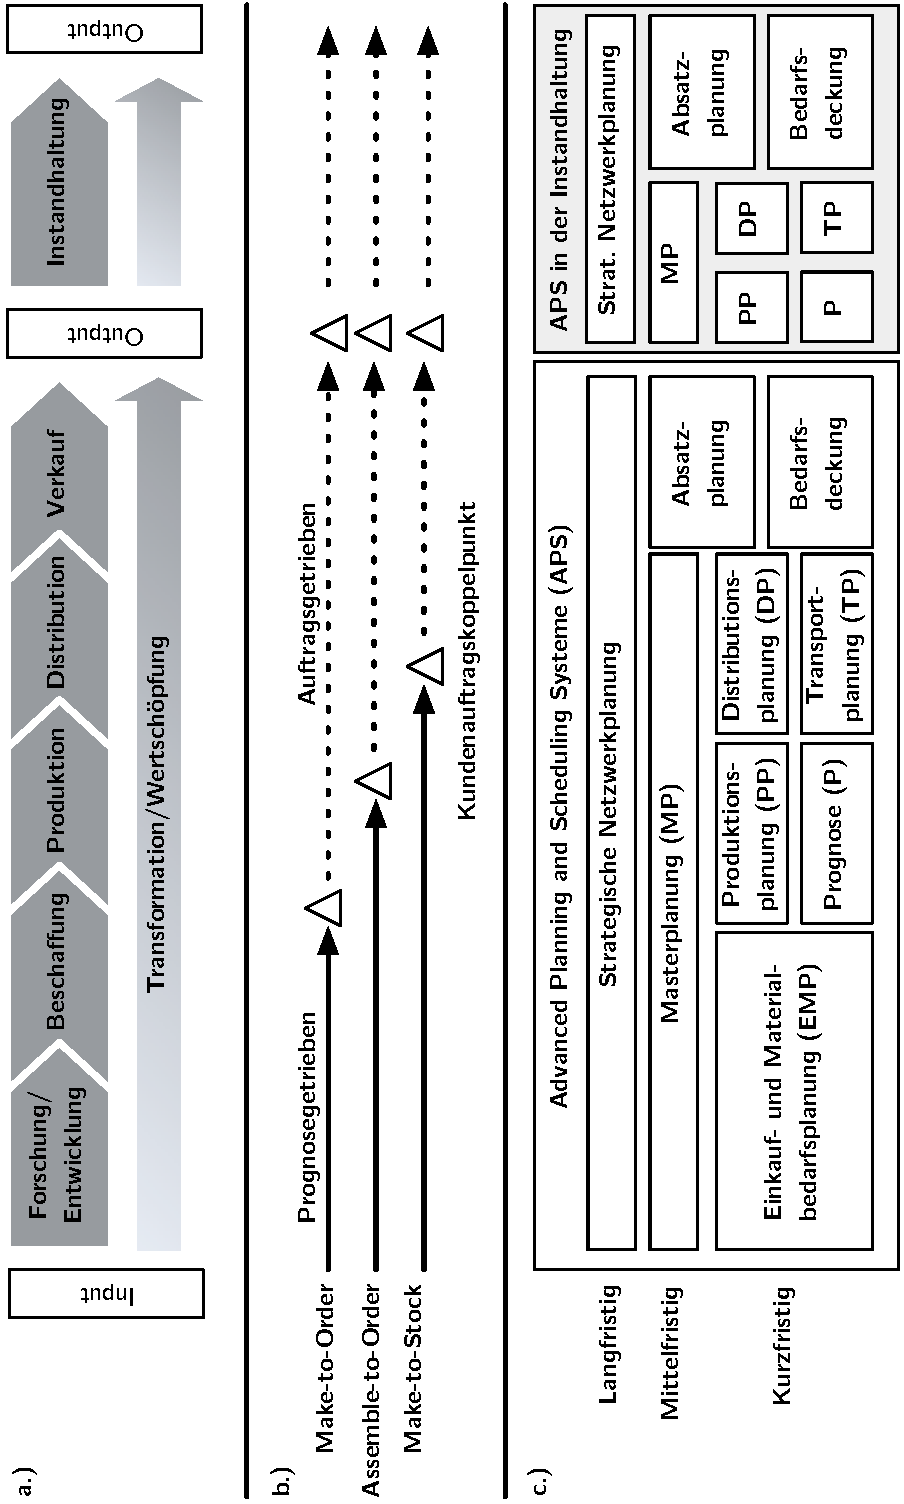
\includegraphics[width=100mm]{Bilder/prozess.pdf}
    \caption{Grafische Veranschaulichung eines Wertschöpfungsprozesses}  \label{Prozess}
    {\footnotesize \textbf{In Anlehnung an:} \cite{quante2009management}, S. 21-22; \cite{Bach:2012aa}, S. 4-5.}
  \end{center}
\end{figure}


Zur Produktionswirtschaft zählt die Planung und Steuerung des Produktionsprogramms und der Produktionsprozesse....



\section{Charakteristika}

\section{Relevanz für betriebliche Entscheidungen}
